

\documentclass{sig-alternate-05-2015}

% Include useful packages
\usepackage{graphicx}
\graphicspath{ {images/} }
\usepackage{float}


\begin{document}

% Copyright
\setcopyright{acmcopyright}


\title{Testing and Tuning SkinnyDip: Noise-Robust Clustering}
\numberofauthors{2} 
\author{
% You can go ahead and credit any number of authors here,
% e.g. one 'row of three' or two rows (consisting of one row of three
% and a second row of one, two or three).
%
% The command \alignauthor (no curly braces needed) should
% precede each author name, affiliation/snail-mail address and
% e-mail address. Additionally, tag each line of
% affiliation/address with \affaddr, and tag the
% e-mail address with \email.
%
% only author :(
\alignauthor
Grant King\\
       \email{kinggra1@msu.edu}
}
% There's nothing stopping you putting the seventh, eighth, etc.
% author on the opening page (as the 'third row') but we ask,
% for aesthetic reasons that you place these 'additional authors'
% in the \additional authors block, viz.
\date{28 April 2017}
% Just remember to make sure that the TOTAL number of authors
% is the number that will appear on the first page PLUS the
% number that will appear in the \additionalauthors section.

\maketitle

\begin{figure*}[t]
\centering
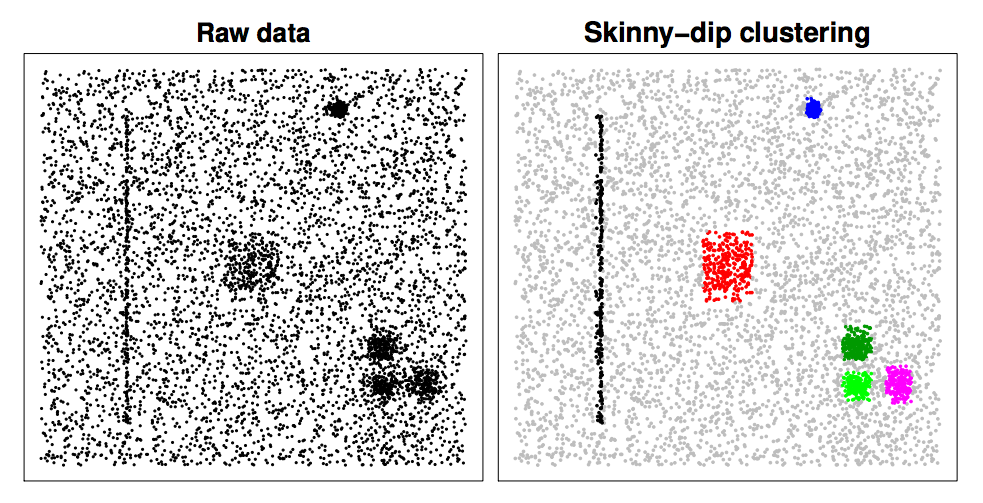
\includegraphics[width=\textwidth]{images/SkinnyDipExample}
\caption{The running example used by Maurus, et al. throughout \cite{skinnydip}}
\label{fig:sdexample}
\end{figure*}

\begin{figure*}[t]
\centering
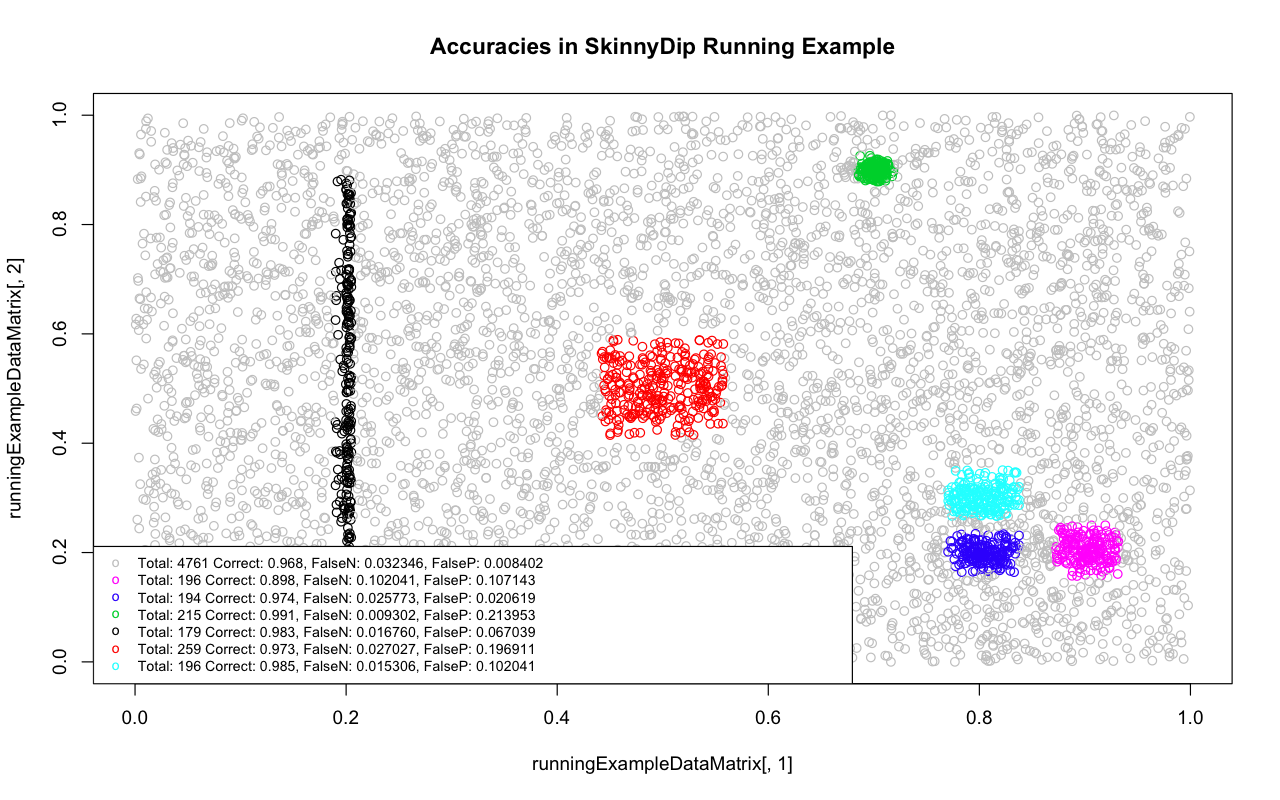
\includegraphics[width=\textwidth]{images/SkinnyDipAccuracy}
\caption{Accuracies of the given SkinnyDip example. NOTE: introduced a bug while updating code that caused legend labels to be shuffled incorrectly, reported data does not correctly match class colors. This will be corrected and updated to a different folder after report has been completed to maintain a "before midnight" commit timestamp.}
\label{fig:sdaccuracy}
\end{figure*}

\section{Problem Description}
It is not uncommon for some real-world data sets to feature an abundance of noise. Depending on the severity of this noise, classical clustering methods may fail due to due to dependence on clean data or confusion from increasingly excessive noise. SkinnyDip is an algorithm proposed by Maurus et al.\cite{skinnydip} designed to handle clustering data in highly noisy environments. SkinnyDip is based on the statistical concept of the \textit{dip} \cite{dip}. 

The dip views the structure of the Empirical Cumulative Distribution Function(ECDF) of a set of single dimensional data to determine whether it is unimodal or multimodal. This test is expanded to a multidimensional, recursive heuristic in order to isolate the various modes of each feature of a set of data. This results in a deterministic, parameter-free, unsupervised method of finding clusters that are based on the modes of multivariate distributions. 

My goal is to augment the SkinnyDip algorithm with the addition of a Gaussian clustering model in an attempt to improve the error that is present in hypercubic-bound clusters, and perform additional tests to demonstrate its usefulness on noisy, real-world data sets.


\section{Introduction}
Data clustering is a fundamental problem in Machine Learning, and has been approached in a variety of ways, resulting in a plethora of tools and methods \cite{ClusteringMethods}, many of which are sensitive to noise and other outliers. Additionally, many common techniques, such as k-means clustering, operate as closed set clustering methods and are unable to reject noise at all.

\cite{DBSCAN} is a density-based technique for finding clusters in environments that may contain noise. However, it has the disadvantages of being a parameterized method, and still continues to find extraneous clusters in increasingly noisy data when compared to SkinnyDip.

A single other existing method for clustering using the statistical dip test was found, a technique called DipMeans\cite{dipmeans}. This method takes a different approach to using the dip test by performing it on a collection of distance measurements as opposed to the raw data values themselves. SkinnyDip, however, requires no distance measurements  and is both functionally and computationally distinct from the DipMeans technique.

While SkinnyDip does manage to find all values within a cluster with high accuracy and precision, there is still a notable risk of falsely matching noise to a particular class. This is inherent in the way that the algorithm segments the clusters into hypercubic regions. If the data does not fit a cubic model, then the values included in extreme regions of the cluster (e.g. the corners of a square cluster) are likely to be false positives and should not have been included. This discrepancy increases exponentially as the dimension of the data increases, an issue acknowledged in the original paper\cite{skinnydip}. I plan to demonstrate that the addition of a second step to clustering can reduce this particular error rate, with minimal negative impact on the existing true positive matches.

\section{Data} \label{data}
A visual example of the purpose of SkinnyDip is demonstrated in the running example data from \cite{skinnydip} (See Figure \ref{fig:sdexample}) which shows the extraction of distinct shapes from a two-dimensional data field that consists of 80\% static noise. A variety of similar clustering methods were shown to perform poorly on this data set, both through the inclusion of the evenly-distributed, static noise in clusters, and through excessive segmentation of the actual classes.

Aside from the uniform background noise, the running example data consists of 2 distinct cluster models: two rectangular model clusters and four 2D Gaussian model clusters. In Figure \ref{fig:sdexample} the square classes are on the left side of the image and are colored red and black, while the remaining four, smaller clusters are the 2D Gaussians. In the process of generating this data, 200 points are generated using their respective distributions (uniform or normal), and placed alongside uniform noise covering the entire field. Any noise that falls within the bounds of these distributions is recategorized as being part of that class.

In the process of testing the existing SkinnyDip results, I created tools to generate Gaussian clusters of arbitrary dimensionality in a field of uniformly random background noise. These were designed to test the inherent error in SkinnyDip's boundaries for normally distributed features, and to further see how this error changed as the dimension of the data increased. For this data, the clusters and background noise were generated, and then any background noise within the ~95\% confidence interval of a cluster (2 standard deviations of the mean) was also classified into that cluster.

Any synthetic or real data that will be analyzed using both the original and my augmented version of SkinnyDip should have uniformly random background noise, or there will be clusters falsely detected by variations in the distribution of the background. The algorithm also benefits from a certain degree of density to the background noise, as an increase in even background noise can help flatten out falsely modal areas of noise.

\section{SkinnyDip}
\subsection{Algorithm}

\subsection{Testing}
My initial hypothesis was that the hypercubic regions returned by the SkinnyDip algorithm would represent an over-classification of noise into the membership of each cluster. As the algorithm returns arbitrary labeled clusters, this first involved finding a way to associate each cluster back to its ground truth membership for comparison. \\

I changed this method to prioritize data point overlap over cluster mean distances. The main motivation of this change was to factor in the actual size of clusters as opposed to just their locations. Additionally, this allows us to confirm whether or not a cluster has successfully been found. Random noise may possibly be falsely classified as a cluster, in which case it will have a meaningful nearest ground truth mean, but the intersection of points in the found and ground truth clusters will not represent the majority of points present in the ground truth cluster. This would indicate that we have found a false cluster relative to the ground truth, but this was not apparent before doing a point-set comparison. In this way, is also possible to set a threshold ratio to determine what is and is not a valid cluster compared to the ground truth. Once the best mapping of detected to ground truth labels had been determined, the SkinnyDip results could be mapped onto the original data and individual label point-sets could be compared. \\

To gather some initial information about the quality of the clusters, I reported a number of statistics about the detected clusters. The reported values included:
\begin{enumerate}
	\item The total number of points placed in the cluster
	\item The percentage of ground truth points detected
	\item The false negative percentage
	\item The false positive percentage
\end{enumerate}
Using these metrics, I expanded upon the authors' reporting by color plotting each of the classified points, and adding a legend with my reported statistics, associated with the respective plot colors. I also wanted to visualize the ground truth values of data I was testing, so I added the option to plot the ground values as well. 


As described in section \ref{data}, the ground truth membership of the synthetic clusters was defined to be the number of points within 2 standard deviations of the cluster mean.
\subsection{Tuning}
As discussed in section \ref{results}, I discovered that the SkinnyDip algorithm was under-classifying valid points into clusters, or equivalently, over-classifying into the noise category from each class. My first idea to correct for this was to incorporate a certain number of nearest adjacent points into a cluster, but I could not think of a good criteria for termination, and realized that this would generally function as inflating the existing cluster in the same hypercubic shape.

My final implementation decision was based on the idea that the contents of these initial cluster regions, although incomplete, would still have information about the underlying structure of the cluster itself.

In my analysis of this synthetic data, it is clear that Gaussian models composed of a large number of false positives, even in just this 2D case. An image analyzing the the classification accuracy of this particular data set is seen in Figure \ref{fig:sdaccuracy}. In this image, the locations of the different clusters are the same, but the coloration has changed slightly, the two leftmost shapes (black and red) are still the rectangularly modeled clusters, and the four, smaller shapes are the 2D Gaussian clusters.

The classes with rectangular models were the only classes that had a false positive rate below 10\%, while the Gaussian modeled classes had false positive ranges that ranged from 10.2\% up to 21.4\%. This supports my hypothesis that the Gaussian modeled clusters would significantly over-sample from their respective classes.








\subsection{Remaining}
Now that I have a tool set to test the accuracy of each cluster's classifications, I plan to expand this testing by adding further dimensions to the existing synthetic data in order to visualize the change in the false positive rate relative to dimension for Gaussian model clusters. This will also be useful for showing the difference in both true positive and false positive changes as I implement a supporting clustering algorithm.
For implementation of a second algorithm, I plan to take the subsets of data that are sectioned off by the hypercubic bounds of SkinnyDip and perform additional clustering. My initial approach will be a simple parameter estimation for the multi-dimensional Gaussian case to see what effect this has on the true and false positive detection as the dimension of the data increases.
Beyond this, I want to apply this clustering to some of the additional data used in the original SkinnyDip experiments, such as clustering of road segments, to see if this addition will further decrease the noise captured in each of those clusters. As a stretch goal, I would be interested in seeing how this algorithm would apply to star mapping data, such as for the purpose of galaxy clustering.




\section{Implementation}



\section{Results} \label{results}
Starting with multivariate Gaussian, single cluster examples, we have a 1D plot of points that has a unimodal cluster centered.

\subsection{Risks}
My algorithm is offline, so points that are initially present in one cluster are accounted for when calculating its covariance, even if they are later reassigned to be in another cluster. This type of conflict will occur when clusters are sufficiently close together or have a sufficiently wide distributions (consider a bimodal distribution that does not reach reach its minimum value between peaks). In this case, the cluster with a higher label in ground truth ordering will take precedence, and all points in the intersection will be assigned to this cluster. Note that this conflict will not occur with the SkinnyDip clusters themselves, they will either be merged, or separate enough that there is no overlap; the conflict only occurs when we try to extend the membership of the cluster.


\section{Future Work}
I believe that the loss at higher dimensions could possibly be reduced by finding an increasing  1


Further analysis of the covariance before reclustering could show relatively uniform noise, indicating that a hypercubic cluster region may actually be a uniform hypercube, as seen in the running example data.


\begin{figure*}[t]
\centering
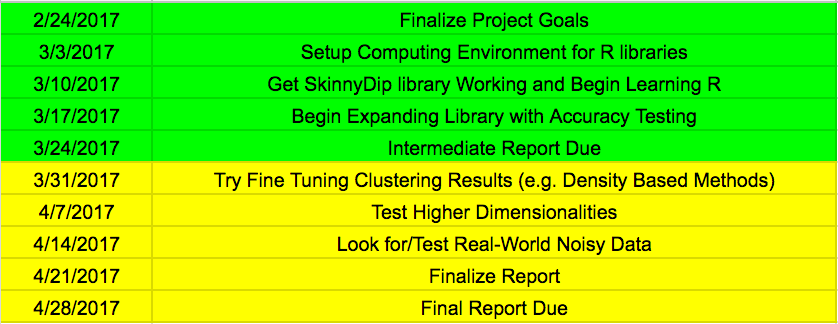
\includegraphics[width=\textwidth]{images/newtimeline}
\caption{Progress on Project Milestones}
\label{fig:newmilestones}
\end{figure*}



\bibliography{final-report}
\bibliographystyle{unsrt}
\end{document}
